% Assignment source: ne630/homework/markdown/HW06.md.
% Legacy foundation: ne630_problems/lesson_06/statement.tex @ e1fba66.
% Problem 1 is new for Fall 2026. Problem 2 adapts legacy Problem 1, and
% Problem 3 adapts legacy Problem 2 to determine the normalization explicitly.

% --------------------------------------------------------------------------
% Problem 1
% --------------------------------------------------------------------------
\noindent{\bf Problem 1}. Use OpenMC's Python nuclear-data interface to
examine the radiative-capture cross section, $\sigma_\gamma(E)$, of
\isoA{U}{238}. No transport calculation is required. On Beocat, the
continuous-energy data file is
\begin{center}
\texttt{/homes/jaroberts/openmc/data/neutron/U238.h5}.
\end{center}
Load this file with \texttt{openmc.data.IncidentNeutron.from\_hdf5}, use the
radiative-capture reaction (ENDF MT 102), and select the \texttt{"294K"}
cross section. The resulting callable takes neutron energy in eV and returns
the microscopic cross section in barns.

\begin{enumerate}[label=(\alph*)]
\item Plot $\sigma_\gamma(E)$ over $10^{-4}\leq E\leq10^7~\mathrm{eV}$
using log--log axes.
\item Above approximately what energy do the individual resonance peaks begin
to overlap and appear as a relatively smooth curve?
\item Plot $\sigma_\gamma(E)$ again over $1\leq E\leq100~\mathrm{eV}$ using
a linear energy axis and a logarithmic cross-section axis.
\item At what energy is the first large resonance peak?
\end{enumerate}
Use energy meshes fine enough to resolve the narrow resonances. Increase the
mesh resolution until the plotted resonance locations and heights no longer
change visibly.

\begin{draftsolution}
I loaded the 294~K, MT-102 cross section directly from the OpenMC HDF5 file.
For example, the data and two plotting meshes can be prepared with
\begin{minted}{python}
import numpy as np
import openmc

data_path = "/homes/jaroberts/openmc/data/neutron/U238.h5"
u238 = openmc.data.IncidentNeutron.from_hdf5(data_path)
sigma_gamma = u238.reactions[102].xs["294K"]

E_full = np.geomspace(1.0e-4, 1.0e7, 500_000)
E_resolved = np.linspace(1.0, 100.0, 1_000_001)
sig_full = sigma_gamma(E_full)
sig_resolved = sigma_gamma(E_resolved)
\end{minted}
The wide-range result is
\begin{center}
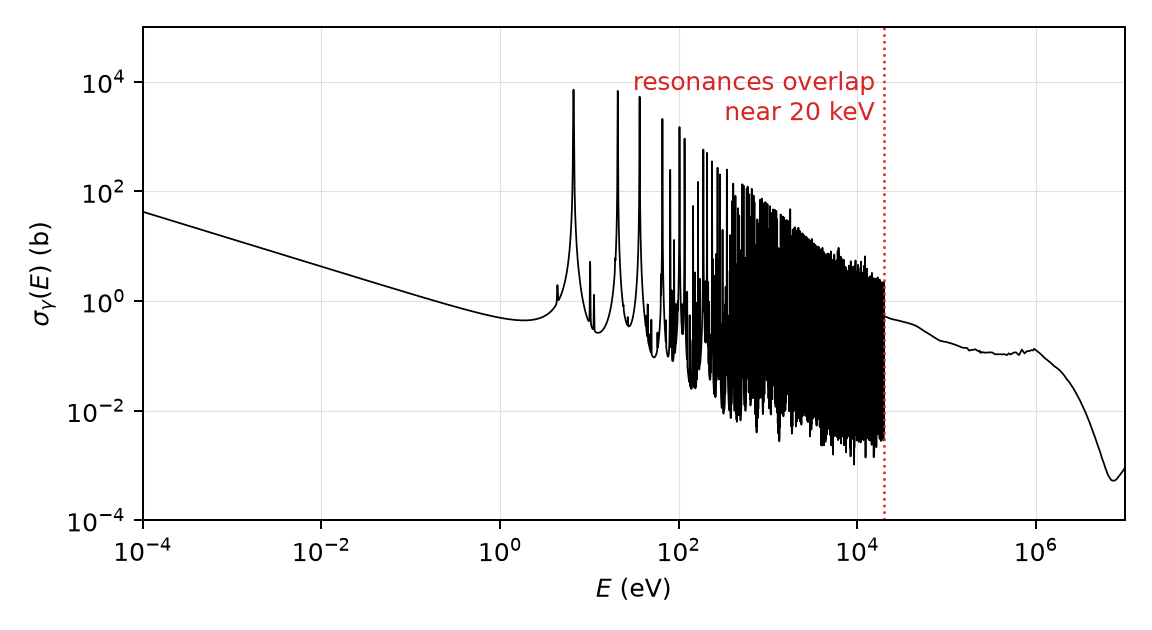
\includegraphics[width=0.86\textwidth]{figures/hw06_u238_capture_full.png}
\end{center}
At low energy, the resonances are well separated. At about
$\boxed{2\times10^4~\mathrm{eV}}$, or $20~\mathrm{keV}$, they begin to
overlap and the evaluated cross section appears relatively smooth on this
scale.

Restricting the energy interval gives
\begin{center}
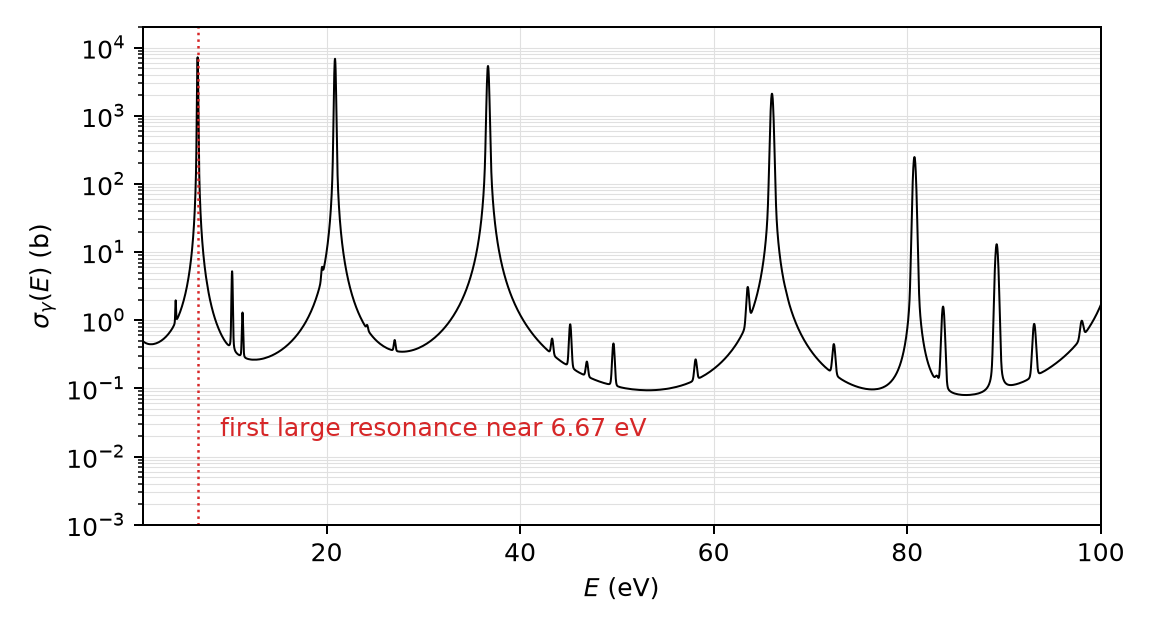
\includegraphics[width=0.86\textwidth]{figures/hw06_u238_capture_1_100ev.png}
\end{center}
The first large resonance is at approximately
$\boxed{E_r=6.67~\mathrm{eV}}$. On the native 294~K tabulation used for the
figure, the local maximum occurs at $6.67428~\mathrm{eV}$; the extra digits
describe the processed energy grid rather than the accuracy with which the
resonance energy should be reported.

I repeated the $1$--$100~\mathrm{eV}$ plot with successively finer uniform
meshes down to $\Delta E\simeq10^{-4}~\mathrm{eV}$. The visible peak
locations and heights no longer changed at the plotting resolution. Using
the native tabulation gives the same plotted result and avoids skipping any
of the energy knots stored in the HDF5 file.
\end{draftsolution}

\newpage

% --------------------------------------------------------------------------
% Problem 2
% The fifth neutron width is 1.874e-3 eV in the Fall 2026 assignment. The
% archived lesson06_sol.ipynb used 1.874e-2 eV; that factor-of-ten typo is not
% propagated here.
% --------------------------------------------------------------------------
\noindent{\bf Problem 2}. Reconstruct the \isoA{U}{238} radiative-capture
cross section over $1\leq E\leq100~\mathrm{eV}$ with the single-level
Breit--Wigner (SLBW) approximation. For resonance $i$,
\[
 \Gamma_i=\Gamma_{n,i}+\Gamma_{\gamma,i},
 \qquad
 \lambda_i=\frac{4.55\times10^{-10}~\mathrm{cm}}
 {\sqrt{E_{r,i}/(1~\mathrm{eV})}},
\]
\[
 \sigma_{0,i}=4\pi\lambda_i^2\frac{\Gamma_{n,i}}{\Gamma_i},
\]
\[
 \sigma_{\gamma,i}(E)
 =\sigma_{0,i}\frac{\Gamma_{\gamma,i}}{\Gamma_i}
 \left(\frac{E_{r,i}}{E}\right)^{1/2}
 \frac{1}{1+4(E-E_{r,i})^2/\Gamma_i^2},
\]
and
\[
 \sigma_\gamma^{\mathrm{SLBW}}(E)=\sum_i\sigma_{\gamma,i}(E).
\]
All energies and widths in these expressions are in eV. The expression for
$\sigma_{0,i}$ produces an area in $\mathrm{cm^2}$; use
$1~\mathrm{b}=10^{-24}~\mathrm{cm^2}$ to report cross sections in barns.
Treat the SLBW reconstruction as a $0~\mathrm{K}$ result.

\begin{center}
\begin{tabular}{rcc}
\toprule
$E_{r,i}$ (eV)&$\Gamma_{n,i}$ (eV)&$\Gamma_{\gamma,i}$ (eV)\\
\midrule
6.67   &$1.476\times10^{-3}$&$2.300\times10^{-2}$\\
20.87  &$1.009\times10^{-2}$&$2.286\times10^{-2}$\\
36.68  &$3.355\times10^{-2}$&$2.300\times10^{-2}$\\
66.03  &$2.418\times10^{-2}$&$2.331\times10^{-2}$\\
80.75  &$1.874\times10^{-3}$&$2.339\times10^{-2}$\\
102.56 &$7.077\times10^{-2}$&$2.408\times10^{-2}$\\
\bottomrule
\end{tabular}
\end{center}
Although the last resonance is centered just above the plotted interval,
include its contribution to the sum.

\begin{enumerate}[label=(\alph*)]
\item Compute and plot $\sigma_\gamma^{\mathrm{SLBW}}(E)$ over
$1\leq E\leq100~\mathrm{eV}$ using a linear energy axis and a logarithmic
cross-section axis.
\item On the same axes, plot the $294~\mathrm{K}$ OpenMC cross section from
Problem 1(c).
\item Compare the two curves. Discuss the resonance locations, peak heights,
peak widths, and any structure not reproduced by the six-resonance SLBW
model. Explain the principal physical reason for the difference in peak
height and width between the $0~\mathrm{K}$ SLBW result and the
$294~\mathrm{K}$ OpenMC data.
\end{enumerate}
Use a sufficiently fine linear energy grid or local refinement near each
resonance, and demonstrate that the reconstructed peaks are converged with
respect to the grid resolution.

\begin{adaptedsolution}
The cross-section values reconstructed from the SLBW approximation are shown
below with values taken from OpenMC. As in the in-class demo, I've used
Python, but Excel or other tools are perfectly acceptable.
\begin{minted}{python}
Er = np.array([6.67, 20.87, 36.68, 66.03, 80.75, 102.56])
Gn = np.array([1.476e-3, 1.009e-2, 3.355e-2,
               2.418e-2, 1.874e-3, 7.077e-2])
Gg = np.array([2.300e-2, 2.286e-2, 2.300e-2,
               2.331e-2, 2.339e-2, 2.408e-2])

E = np.linspace(1.0, 100.0, 1_980_001)  # Delta E = 5e-5 eV
sigma_slbw = np.zeros_like(E)
for Er_i, Gn_i, Gg_i in zip(Er, Gn, Gg):
    Gamma_i = Gn_i + Gg_i
    lambda_i = 4.55e-10/np.sqrt(Er_i)
    sigma_0_i = 4*np.pi*lambda_i**2*Gn_i/Gamma_i
    sigma_slbw += (1.0e24*sigma_0_i*(Gg_i/Gamma_i)
                   * np.sqrt(Er_i/E)
                   / (1.0 + 4.0*(E-Er_i)**2/Gamma_i**2))
\end{minted}

\begin{center}
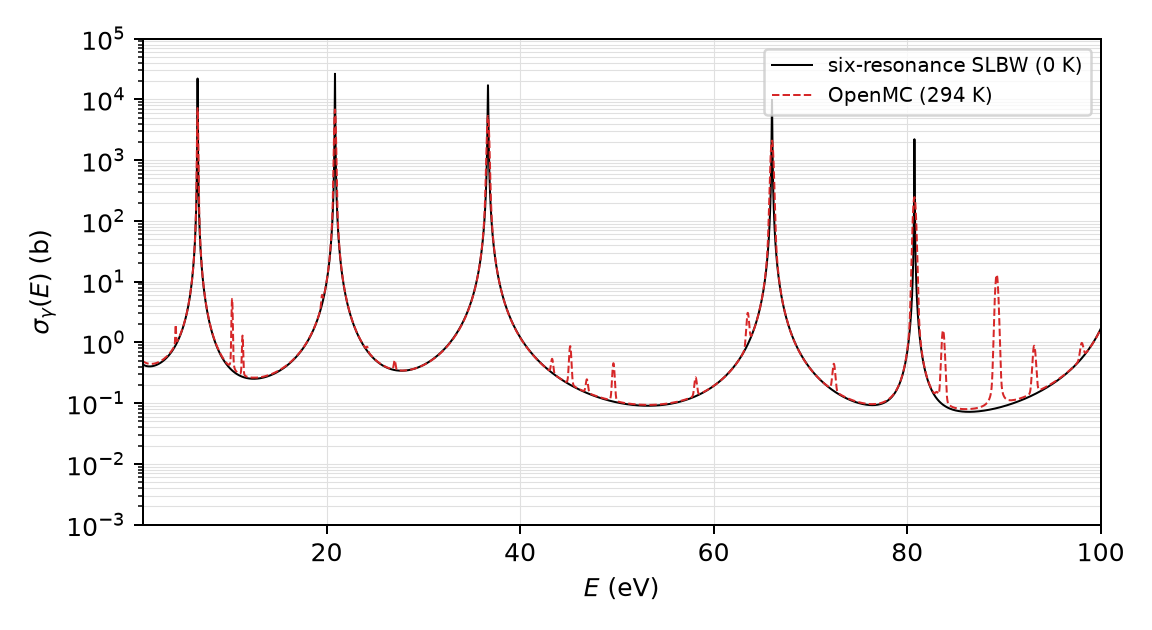
\includegraphics[width=0.88\textwidth]{figures/hw06_slbw_comparison.png}
\end{center}

Overall, the SLBW values are quite close in resonance location for the five
principal resonances exhibited in the energy range. Representative peak and
width values are
\begin{center}\small
\begin{tabular}{rrrr}
\toprule
$E_r$ (eV)&$\Gamma$ (eV)&SLBW peak (b)&294~K OpenMC peak (b)\\
\midrule
6.67  &0.024476&22103&7196\\
20.87 &0.032950&26483&6838\\
36.68 &0.056550&17114&5358\\
66.03 &0.047490& 9847&2101\\
80.75 &0.025264& 2213& 247\\
\bottomrule
\end{tabular}
\end{center}
For an isolated SLBW resonance, the full width at half maximum is
approximately $\Gamma$. The corresponding widths read from the 294~K curve
are about $0.103$, $0.176$, $0.240$, $0.306$, and $0.323~\mathrm{eV}$,
respectively. Thus, the SLBW values exhibit narrower and taller resonances
than the OpenMC data.

The six-resonance sum is also missing fine detail and background structure
that cannot be captured by this model. Recall from class that the OpenMC data
are provided at 294~K. On the other hand, the SLBW model here provides values
for 0~K. The increased temperature leads to \emph{Doppler broadening}, which
spreads each resonance over a wider energy interval and lowers its peak while
approximately preserving its resonance area. The 102.56-eV resonance must be
included even though its center lies outside the plot: at $100~\mathrm{eV}$,
its tail contributes $1.669~\mathrm b$ of the $1.677~\mathrm b$ SLBW total.

I reduced the uniform SLBW grid spacing from $10^{-3}$ to
$5\times10^{-5}~\mathrm{eV}$. The resonance locations and quoted peak
heights were unchanged at the shown precision, and the plotted curves were
visually indistinguishable. The final grid places about 490 points across
even the narrowest total resonance width.
\end{adaptedsolution}

\newpage

% --------------------------------------------------------------------------
% Problem 3
% Numerical values reproduce the legacy approach but normalize the spectrum
% before evaluating either requested probability.
% --------------------------------------------------------------------------
\noindent{\bf Problem 3 [adapted from FNRP 2.9]}. The fission-neutron energy
spectrum is modeled by
\[
 \chi(E)=C\exp(-1.036E)\sinh\!\left(\sqrt{2.29E}\right),
 \qquad E\geq0,
\]
where $E$ is in MeV, $\chi(E)$ is a probability density per MeV, and $C$ is
an unknown normalization constant. Use numerical integration and the
normalized form of $\chi(E)$ to determine the following. Report $C$ and each
fraction to at least three significant figures.

\begin{enumerate}[label=(\alph*)]
\item Evaluate the required integral over the whole domain,
$0\leq E<\infty$, and determine $C$ such that
\[
 \int_0^\infty\chi(E)\,dE=1.
\]
\item Evaluate the fraction of fission neutrons born with energies in
$0\leq E\leq0.1~\mathrm{MeV}$.
\item Evaluate the fraction of fission neutrons born with energies in
$10~\mathrm{MeV}\leq E<\infty$.
\end{enumerate}
Integrate over each stated interval directly. If the numerical method
replaces $\infty$ with a finite upper limit, demonstrate that the result has
converged as that limit is increased.

\begin{adaptedsolution}
The distribution of fission-neutron energies is modeled by
\[
 \chi(E)=C\exp(-1.036E)\sinh(\sqrt{2.29E}),
\]
where $E$ is in MeV. This is definitely a problem best solved using a
numerical technique. Here, I'm using \texttt{scipy.integrate.quad}:
\begin{minted}{python}
import numpy as np
from scipy.integrate import quad

g = lambda E: np.exp(-1.036*E)*np.sinh(np.sqrt(2.29*E))
I = quad(g, 0.0, np.inf)[0]
C = 1.0/I
chi = lambda E: C*g(E)

p_below = quad(chi, 0.0, 0.1)[0]
p_above = quad(chi, 10.0, np.inf)[0]
\end{minted}

\begin{enumerate}[label=(\alph*)]
\item The unnormalized integral is
\[
 I=\int_0^\infty
 \exp(-1.036E)\sinh(\sqrt{2.29E})\,dE
 \approx2.210125128.
\]
Therefore,
\[
 \boxed{C=\frac{1}{I}\approx0.452463070~\mathrm{MeV^{-1}}}.
\]

\item Direct integration over the requested interval gives
\[
 \int_0^{0.1}\chi(E)\,dE
 \approx\boxed{0.0138794},
\]
or about $1.39\%$ of the fission neutrons.

\item Direct integration over the high-energy tail gives
\[
 \int_{10}^{\infty}\chi(E)\,dE
 \approx\boxed{0.00106030},
\]
or about $0.106\%$ of the fission neutrons.
\end{enumerate}

As a finite-upper-limit check, using upper limits of 20, 30, and 40~MeV for
the high-energy-tail integral gives $0.00106008$, $0.00106030295$, and
$0.00106030298$, respectively. Likewise, the normalized integral over
$0\leq E\leq40~\mathrm{MeV}$ is $0.99999999999996$. The reported values are
therefore converged well beyond the requested three significant figures.
\end{adaptedsolution}

\clearpage
